% IEEEtran initializes legacy Times metrics before fontspec enables Unicode text.
\def\encodingdefault{OT1}
\documentclass[journal]{IEEEtran}
\usepackage{iftex}
\ifPDFTeX
  \usepackage[T1]{fontenc}
  \usepackage{microtype}
\else
  \usepackage{fontspec}
  \setmainfont{texgyretermes}[
    Extension=.otf,
    UprightFont=*-regular,
    BoldFont=*-bold,
    ItalicFont=*-italic,
    BoldItalicFont=*-bolditalic]
  \usepackage[expansion=false]{microtype}
\fi
\usepackage{amsmath}
\usepackage{array}
\usepackage{booktabs}
\usepackage{graphicx}
\usepackage{placeins}
\usepackage{xurl}
\newcommand{\pending}[2]{\par\smallskip\noindent\textbf{Pending [#1].} #2\par\smallskip}

\title{Supplementary Material: Cross-Map Representation and Generalization of Defensive Openings in Counter-Strike 2}
\author{Working draft: author details pending}
\renewcommand{\thetable}{S\arabic{table}}
\renewcommand{\thefigure}{S\arabic{figure}}
\begin{document}
\maketitle
\noindent This separate supplement retains input ablations, context sensitivity, supporting audits and reproducibility details. All results and author-review limitations belong to the same working study.
\appendices

\section{Input Ablations and Context Sensitivity}
\label{app:ablations}
The four core architecture conditions remain in the main comparisons. The following two conditions reduce inputs only within the graph-temporal architecture; they are not extra architectures or independent samples. All targets, masks and selection rules remain unchanged.

\begin{table}[!h]
\caption{Development input ablations. The full-input Graph+GRU reference is in main-paper Table~IV; all entries reconstruct the same target.}
\label{tab:inputablation}
\centering\small
\begin{tabular}{lrr}
\toprule
Condition & G3 loss & G4 loss\\
\midrule
Graph + GRU, no motion & 0.096085 & 0.126011 \\ % [claim:C134] [evidence:E110]
Graph + GRU, common input & 0.096766 & 0.125923 \\ % [claim:C135] [evidence:E110]
\bottomrule
\end{tabular}
\end{table}

Adding motion to the specified graph-temporal architecture reduced the G3 objective by 3.87\%, with descriptive interval [1.45, 6.01]\%. The G4 reduction was 0.49\%, with interval [-0.68, 1.60]\%, so this development experiment does not establish a reliable cross-map motion gain. Input-ablation results are conditional on this architecture. % [claim:C126] [evidence:E110]

\begin{table*}[t]
\caption{Input-ablation pattern diagnostics. The full-input reference and eligibility definitions are in main-paper Table~V.}
\label{tab:patternablation}
\centering\small
\begin{tabular}{lrrrr}
\toprule
Condition & G3 ARI & G4 ARI & G4 pairs & Coverage (\%)\\
\midrule
Graph + GRU, no motion & 0.586 & 0.346 & 16/18 & 89.5 \\ % [claim:C144] [evidence:E114]
Graph + GRU, common input & 0.387 & 0.566 & 18/18 & 85.0 \\ % [claim:C145] [evidence:E114]
\bottomrule
\end{tabular}
\end{table*}

\begin{table}[t]
\caption{New-series input ablations. The full-input reference is in main-paper Table~VII; losses are descriptive secondary results.}
\label{tab:newablation}
\centering\small
\begin{tabular}{lr}
\toprule
Condition & Mean loss\\
\midrule
Graph + GRU, no motion & 0.124499 \\ % [claim:C178] [evidence:E131]
Graph + GRU, common input & 0.125665 \\ % [claim:C179] [evidence:E131]
\bottomrule
\end{tabular}
\end{table}

\begin{figure*}[t]
\centering
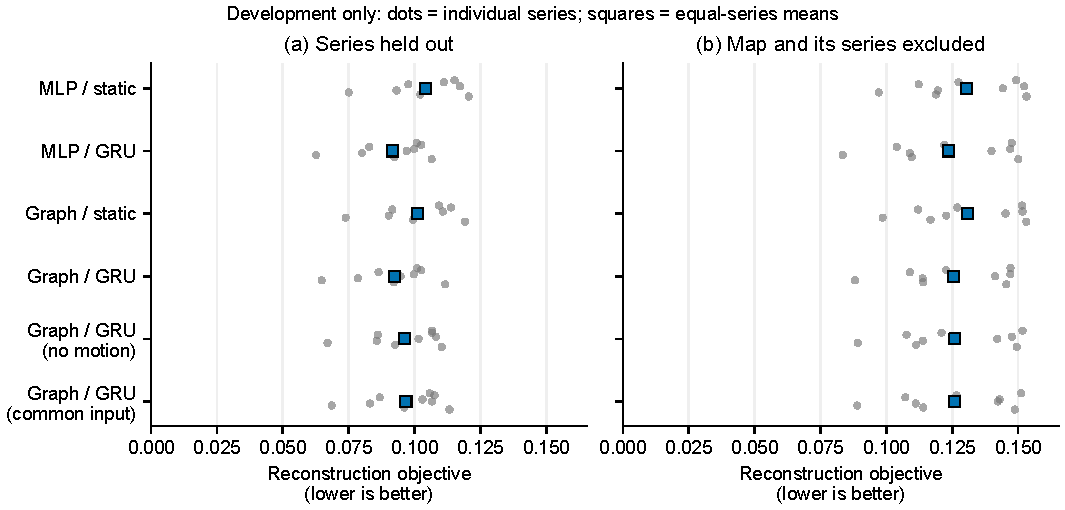
\includegraphics[width=\textwidth]{figures/reconstruction.pdf}
\caption{Development reconstruction by series. Each dot averages the three neural seeds within windows and then the windows within one series; the square is the equal-series mean. The panels use a common objective scale. These are descriptive development observations, not independent tactical judgments.}
\label{fig:reconstruction}
\end{figure*}

\subsection{Context components and weight sensitivity}
\label{app:contextpolicies}
Single-group controls and the prespecified weights probe different context contributions. They are separated from the core graph/nongraph and static/temporal comparisons.

We retain the frozen state encoders and add explicit CT context: five log equipment totals, two public pre-round scores, and thirty log throw counts over the five times and six grenade types, for 37 coordinates. Equipment reweights information already present in the node input; score and recorded utility supply additional observations. Opponent equipment and raw view angles are excluded. % [claim:C150] [evidence:E121]

\begin{table}[t]
\caption{New-series unjudged retrieval turnover. Counts pool twenty method/seed variants, not independent participants. Utility-dependent policies use the 245 context-known windows. Changing the first result is not evidence of improved relevance.}
\label{tab:transferretrieval}
\centering\small
\setlength{\tabcolsep}{4pt}
\begin{tabular}{lrr}
\toprule
Policy & Queries & Top-1 changes/comparisons\\
\midrule
Base & 246 & 0/4920 \\ % [claim:C193] [evidence:E151]
CT equipment & 246 & 2408/4920 \\ % [claim:C194] [evidence:E151]
Public score & 246 & 3892/4920 \\ % [claim:C195] [evidence:E151]
CT utility & 245 & 4112/4900 \\ % [claim:C196] [evidence:E151]
Joint context, 0.25 & 245 & 3084/4900 \\ % [claim:C197] [evidence:E151]
Joint context, 0.50 & 245 & 4007/4900 \\ % [claim:C198] [evidence:E151]
Joint context, 0.75 & 245 & 4509/4900 \\ % [claim:C199] [evidence:E151]
\bottomrule
\end{tabular}
\end{table}

\section{Supporting Audits and Auxiliary Prediction}
\label{app:supporting}
\subsection{Component and observation audits}
The G4 Nuke diagnostic contains 62 windows from three series. Full Graph + GRU has 8.44\% higher loss than MLP + GRU and 3.72\% higher loss than its common-input control. Against the common-input control, the total loss reduction is $-0.003703$, with the region group contributing $-0.003193$ after division by seven. Against the no-motion control, the largest negative contribution is instead the ground-state group ($-0.003691$). These post-hoc component differences use the fixed CE/MSE scales and model-specific optimal player matchings; they do not identify a causal input-field failure. % [claim:C146] [evidence:E117]

A separate context audit reread the same 22 development demos without changing any encoder input. It recovered pre-round scores for all 465 windows, CT and T equipment totals at all 2,325 query times, and finite angle pairs for all 11,368 live CT observations. Dead-player angle slots are masked. This establishes field availability, not improved representation or tactical generalization. % [claim:C147] [evidence:E118]

Throw counts start at freeze end and stop at each query tick; they count recorded releases rather than active smoke or fire effects. Previous outcomes are restricted to completed earlier rounds, with score attributed to stable team identities across side switches. Opponent equipment is privileged observer information, and recorded view direction alone does not establish visibility or tactical duty. These fields remain outside the frozen common encoder input. % [claim:C148] [evidence:E118,E119]

The unchanged six fixed query cases now have CT-only equipment, score and throw-count sidecars. All six queries are first-round windows under the original first-in-index selection rule, so their resource conditions are not representative of the full cohort. Context differences are observable, but neither agreement nor disagreement supplies a tactical relevance judgment. % [claim:C149] [evidence:E120]


\subsection{Auxiliary state prediction}
\label{app:auxprediction}
The completed v17 non-graph control reads the full masked node matrix, distance matrix, and alive mask. It averages a shared MLP over all 120 joint player permutations, preserving edge-endpoint correspondence in every input. Static and causal-GRU prediction variants were compared under the recorded development recipe.

Table~\ref{tab:aux} reports the completed v17 development comparison using the original common inputs and masks. Values are equal-series relative MSE reductions against persistence. Neural scores average errors over seeds 0, 1, and 42; they are not a prediction ensemble.

\begin{table}[t]
\caption{Completed auxiliary development prediction, E6. Relative MSE reduction against persistence (\%). These values do not measure tactical relevance or the revised main representation.}
\label{tab:aux}
\centering
\begin{tabular}{lrr}
\toprule
Method & G3 & G4\\
\midrule
Ridge & 18.06 & 14.71 \\
Graph & 14.51 & 12.07 \\
Graph + GRU & 16.76 & 11.46 \\
Full-input MLP & 15.88 & 13.03 \\
Full-input MLP + GRU & 17.07 & 10.80 \\
\bottomrule
\end{tabular}
\end{table}

The new non-graph conditions did not establish a stable advantage over ridge. This result bounds the current predictive probe; it neither validates the revised deployment representation nor rules out graph usefulness for the original pattern task. The full v7 and v14 controls, paired descriptive intervals, seeds, and failures remain in the evidence supplement.


\section{Evidence and Reproducibility}
Recorded auxiliary evidence is in
\path{datasets/evaluation/ct_information_control_v17_report.json}.
Geometry coverage is in
\path{datasets/evaluation/ct_geometry_features_v17_report.json}.
Cohort and historical protocols are linked in the manuscript writing guide. Raw Demos, human returns, environments, and most weights remain local; the public summaries alone are not a fresh-clone training dataset.

A local CPU reference bundle contains 124 checksummed payload files, including 108 cached prediction archives and six sample indices. Its independently extracted copy reproduces 216 series/condition/seed records, all twelve series summaries, and both primary intervals within absolute tolerance $10^{-10}$. This replays aggregation from cached losses; it does not recompute decoder losses, model inference, training or raw observations. The installed software environments and executable routes are recorded separately. % [claim:C217] [evidence:E145,E146,E148]

The reproducibility guide distinguishes cached-loss replay, frozen-checkpoint inference, from-scratch training, native parsing and the private old-judgment audit. Model weights, training inputs and original human returns are not in the numerical bundle. The local artifact has not been approved for redistribution or anonymous submission; the software license does not establish rights to every underlying material.

\pending{REPRO}{Author review remains necessary for permitted redistribution, anonymized review artifacts and access conditions for raw/native/training materials. The local numerical replay and source entry points are prepared; this is not a claim of complete public reproduction.}
\subsection{Research workflow assistance}
Scientific Agent Skills~\cite{kassis2026skills} informed evidence organization, paired observational comparisons, precision planning and citation checks. The earlier scientific-writing installation was recorded at repository revision \path{593377bb048752abb0152deab9fbb1083a6087df}; current procedural files are recorded separately by content hash, without asserting the same upstream revision for all files. This is workflow assistance, not independent validation of sources, models, or scientific conclusions. % [claim:C107] [evidence:E106,E128]

\section{Telemetry Compatibility}
\label{app:telemetry}
A version-sensitivity probe reparsed one unchanged May Dust2 Demo with demoparser2 0.42.1 instead of 0.41.3. The dedicated throw event remained unavailable, while opening snapshots, timing audits and all five model-input arrays matched exactly. This single-file result does not determine whether recording differences or a remaining compatibility issue causes the event gap, and it does not validate other parser-version substitutions. % [claim:C189] [evidence:E138]

On one October Dust2 control, all 535 paired dedicated releases occur 6--14 game ticks after firing and exactly at the first observed projectile tick; firing timestamps are not interchangeable with releases. After the conservative correction, all 330,660 candidate positions supported in the preceding context version and 4,766 previously known prototype assignments retain their candidate identities or cluster labels and acceptance, with distances checked to absolute tolerance $10^{-10}$. These are telemetry and replay checks, not semantic judgments. % [claim:C200] [evidence:E139,E153]

Native fields distinguish firing from completed release: in one unmatched T-side Molotov action, a positive planned throw time follows pin release, but the owner dies before that time, outside all query windows. Across eight dedicated-event controls, 3,553 normal releases and 830 CT query counts match. Two smoke projectiles instead appear at owner death without a started release or dedicated throw event. These smoke counterexamples are not extrapolated to the unmatched target HE projectile, whose affected counts remain unknown. % [claim:C221] [evidence:E149,E150]

\section{Declarations and Pilot Sources}
\pending{DECL}{Before submission, supply factual author contributions, applicable participant/consent information for any human evidence actually used, data/code availability, funding/conflicts if applicable, and the venue-required AI assistance disclosure. No approval, consent, authorship, or funding statement is invented here.}

\bibliographystyle{IEEEtran}
\bibliography{references}
\end{document}
